%%%%%%%%%%%%%%%%%%%%%%%%%%%%%%%%%%%%%%%%%%%%%%%%%%%%%%%%%%%%%%%%%%%%%%%%%%%%%%%%%%%
%                        Projet série temporelle sorry Arima
%%%%%%%%%%%%%%%%%%%%%%%%%%%%%%%%%%%%%%%%%%%%%%%%%%%%%%%%%%%%%%%%%%%%%%%%%%%%%%%%%%%



% Deze template is gemaakt door Fons van der Plas (f.vanderplas@student.ru.nl) voor het publiek domein en mag gebruikt worden **zonder vermelding van zijn naam**.
% This template was created by Fons van der Plas (f.vanderplas@student.ru.nl) for the public domain, and may be used **without attribution**.
\documentclass{article}
\usepackage[utf8]{inputenc}     % for éô
\usepackage[T1]{fontenc}
\usepackage[french]{babel}     % for proper word breaking at line ends
\usepackage[a4paper, left=1.5in, right=1.5in, top=1.5in, bottom=1.5in]{geometry}
                                % for page size and margin settings
\usepackage{graphicx}           % for ?
\usepackage{amsmath,amssymb}    % for better equations
\usepackage{amsthm}             % for better theorem styles
\usepackage{mathtools}          % for greek math symbol formatting
\usepackage{enumitem}           % for control of 'enumerate' numbering
\usepackage{listings}           % for control of 'itemize' spacing
\usepackage{todonotes}          % for clear TODO notes
\usepackage{hyperref}           % page numbers and '\ref's become clickable

\usepackage{amsmath}
\usepackage{amsfonts}
\usepackage{amssymb}
\usepackage{calrsfs}
\usepackage[mathscr]{euscript}
\usepackage[final]{pdfpages}
%%%%%%%%%%%%%%%%%%%%%%%%%%%%%%%%
\def\thesistitle{Using Bayesian approach in Time Series}
\def\thesissubtitle{Sorry ARIMA, but I’m Going Bayesian}
\def\thesisauthorfirst{Pierre}
\def\thesisauthorsecond{Gauthier}
%\def\thesissupervisorfirst{dr. Dewey}
%\def\thesissupervisorsecond{Duck}
%\def\thesissecondreaderfirst{prof. dr. Louie}
%\def\thesissecondreadersecond{Duck}
\def\thesisdate{9 Décembre 2019}
%%%%%%%%%%%%%%%%%%%%%%%%%%%%%%%%

%% FOR PDF METADATA
\title{\thesistitle}
\author{\thesisauthorfirst\space\thesisauthorsecond}
\date{\thesisdate}

%% TODO PACKAGE
\newcommand{\towrite}[1]{\todo[inline,color=yellow!10]{TO WRITE: #1}}

%% THEOREM STYLES
\newtheorem{theorem}{Theorem}[section]
\newtheorem{corollary}{Corollary}[theorem]
\newtheorem{lemma}[theorem]{Lemma}
\newtheorem{proposition}[theorem]{Proposition}

\theoremstyle{definition}
\newtheorem{definition}[theorem]{Definition}

\theoremstyle{remark}
\newtheorem*{remark}{Remark}


%% MATH OPERATORS
\DeclareMathOperator{\supersine}{supersin}
\DeclareMathOperator{\supercosine}{supercos}

%%%%%%%%%%%%%%%%%%%%%%%

\begin{document}

\begin{titlepage}	
	\thispagestyle{empty}
	\newcommand{\HRule}{\rule{\linewidth}{0.5mm}}
	\center
	\textsc{\Large École des Mines de Nancy}\\[.7cm]

	
	\begin{figure}[h]
		\centering
		\begin{minipage}{.5\textwidth}
			\centering
			
\includegraphics[width=25mm]{logos/logo.png}\\[.5cm]
		\end{minipage}%
		\begin{minipage}{0.5\textwidth}
			\centering
			
\includegraphics[width=25mm]{logos/univ.png}\\[.5cm]
		\end{minipage}
	\end{figure}


%	\textsc{Faculty of Science}\\[0.5cm]
	
	\HRule \\[0.5cm]
	{ \huge \bfseries \thesistitle}\\[0.1cm]
	\textsc{\thesissubtitle}\\
	
	\HRule \\[3cm]
	\begin{minipage}{0.4\textwidth}
		\begin{flushleft} \large
			\emph{Author:}\\
			\thesisauthorfirst\space \textsc{\thesisauthorsecond}
		\end{flushleft}
	\end{minipage}
	~
	\begin{minipage}{0.4\textwidth}
		\begin{flushright} \large
			\textsc{\large Tuteur : Denis Villemonais}\\[.5cm]
	\end{flushright}
\end{minipage}\\[4cm]

{\large \thesisdate}\\
\clearpage
\end{titlepage}

%\emph{Supervisor:} \\
%\thesissupervisorfirst\space \textsc{\thesissupervisorsecond} \\[1em]
%\emph{Second reader:} \\
%\thesissecondreaderfirst\space \textsc{\thesissecondreadersecond}

\tableofcontents

\newpage
{\textbf{\Huge Introduction \\}}

\paragraph{}
Nous allons dans le présent travail explorer les solution présentées par le post de Kim Larsen sur le blog de 
\textit{MultiThreaded} \cite{sorryarima}. 
Les résultats de ce post s'appuient fortement sur \cite{pedictbayesian}.

\paragraph{}
Nous allons tout d'abord présenter les méthodes de prédiction usuelles ARIMA pour ensuite étudier l'approche bayésienne.

\newpage
%%%%%%%%%%%%%%%%%%%%%%%%%%%%%%%%%%%%%%%%%%%%%%%%%%%%%%%%%%%%%%%%%%%%%%%%%%%%%%%%%%%%%%%%%%%%%%%%%%%%%%%%%%%
%%%%%%%%%%%%%%%%%%%%%%%%%%%%%%%%%%%%%%%%%%%%%%%%%%%%%%%%%%%%%%%%%%%%%%%%%%%%%%%%%%%%%%%%%%%%%%%%%%%%%%%%%%%

%%%%%%%%%%%%%%%%%%%%%%%%%%  ARIMA %%%%%%%%%%%%%%%%%%%%%%%%%%%%%%%%%%%%%%%%%%%%%%%%%%%%%%%%%%%%%%%%%%%%%%%%%

%%%%%%%%%%%%%%%%%%%%%%%%%%%%%%%%%%%%%%%%%%%%%%%%%%%%%%%%%%%%%%%%%%%%%%%%%%%%%%%%%%%%%%%%%%%%%%%%%%%%%%%%%%%
%%%%%%%%%%%%%%%%%%%%%%%%%%%%%%%%%%%%%%%%%%%%%%%%%%%%%%%%%%%%%%%%%%%%%%%%%%%%%%%%%%%%%%%%%%%%%%%%%%%%%%%%%%%
\section{Modèlisation avec les processus ARIMA}

\subsection{Généralités sur les séries temporelles}
\paragraph{}
Nous allons rappeler brièvement des éléments du cours de modélisation des séries temporelles par des modèles ARIMA 
tels que introduits par F. Sur \cite{courssur}.

\paragraph{}
On définit tous d'abord une série temporelles par une suite d'observation d'une variable $X_t$ au cours du temps comme sur 
la figure \ref{airmiles}
\begin{figure}[h]
	\label{airmiles}
	\centering
	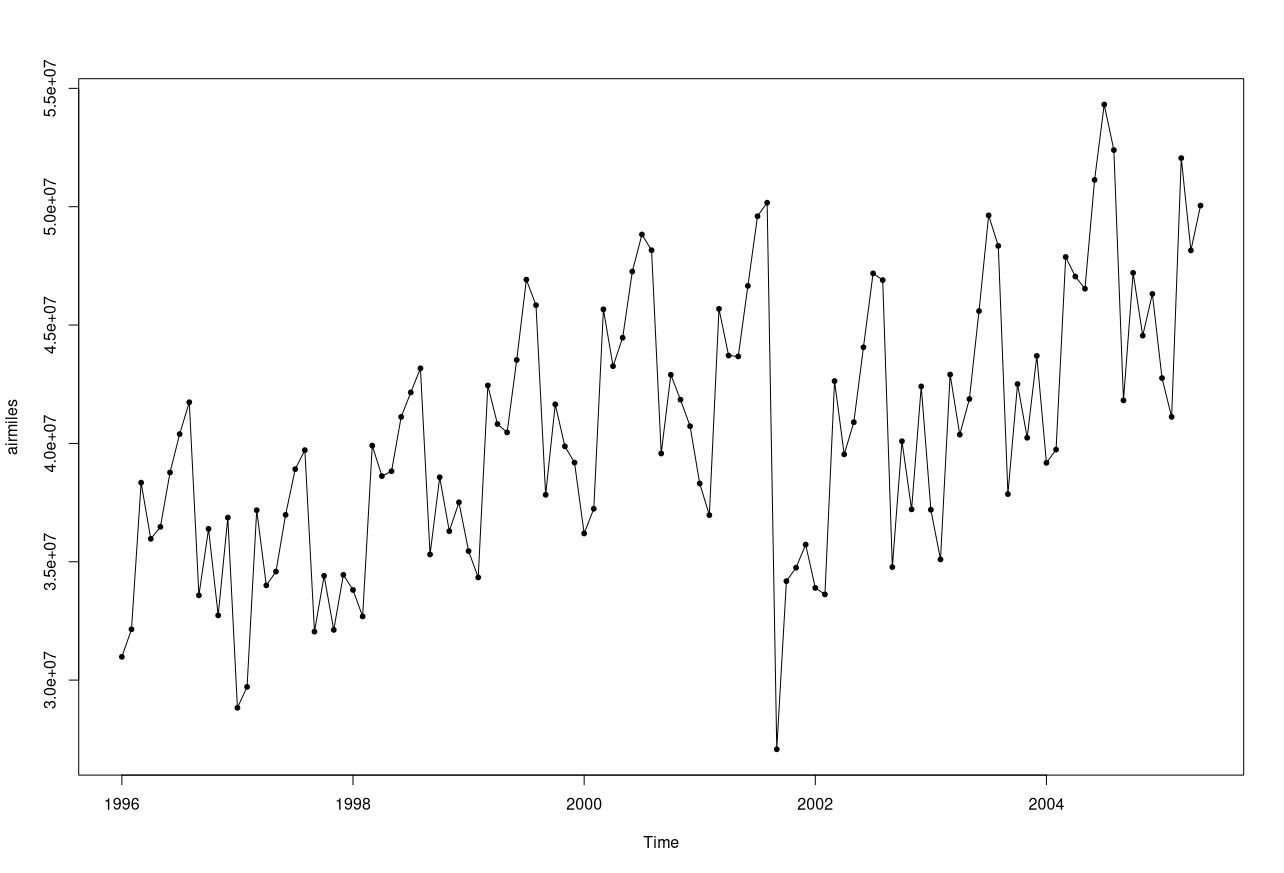
\includegraphics[width=0.5\paperwidth]{logos/airmiles.png}
	\caption{chronique \textit{airmiles} du package \textit{TSA} qui donne le nombre de passagers transportés sur les lignes
	 aériennes aux USA de janvier 1996 à mai 2007}
\end{figure}
\paragraph{}
Un processus aléatoire d'une suite de variable $(X_1, \ldots, X_T)$ est stationnaire au second ordre si il vérifie
les propriétés suivantes:
\[
	\begin{aligned}
		\left\{
			\begin{array}{l}
				{\forall t, \mathbb{E}\left(X_{t}\right)=m \quad \text{(moyenne constante)}}  \\ 
				{\forall (t, s) \ \operatorname{cov}\left(X_{t}, X_{s}\right)=\gamma(|t-s|), \quad \text{(autocovariance symétrique, invariante par translation)}}  \\ 
				{\forall t, \operatorname{var}\left(X_{t}\right)=\gamma(0) \  \text{(homoscédasticité)}} 
			\end{array}
			\right.
\end{aligned}
\]
\paragraph{}
Un bruit blanc gaussien avec des variable $(\epsilon_t)$ i.i.d est un cas particulier de bruit blanc fort vérifiant:
\[
	\begin{aligned}
		\left\{
			\begin{array}{l}
				{\forall t, \mathbb{E}\left(\epsilon_{t}\right)=0}  \\ 

				{\forall t, \operatorname{Var}\left(\epsilon_{t}\right)=\sigma^2} 
			\end{array}
			\right.
\end{aligned}
\]
\paragraph{Autocorrélation ACF\\}
On définit pour l'étude des séries temporelles le coefficient d'autocorrection $\rho(h)$ dit aussi ACF (\textit{auto-correlation function}):
\[
\forall h \geqslant 0, \rho(h)=\frac{\operatorname{Cov}\left(X_{t}, X_{t+h}\right)}{\sqrt{\operatorname{Var}\left(X_{t}\right) \operatorname{Var}\left(X_{t+h}\right)}}=\frac{\gamma(h)}{\gamma(0)}
\]
On utilise en pratique le corrélogramme empirique $\widehat{\rho}(h)$ pour identifier les propriétés de la série temporelle
\begin{equation}
	\widehat{\rho}(h)=\frac{T}{T-h} \frac{\sum_{t=h+1}^{T}\left(X_{t}-\bar{X}_{T}\right)\left(X_{t-h}-\bar{X}_{T}\right)}{\sum_{t=1}^{T}\left(X_{t}-\bar{X}_{T}\right)^{2}}
\end{equation}
\paragraph{Autocorrélation partielle PACF\\}
Dans l'idée d'un modèle auto-projectif nous construisons une prévision linéaire sur la valeur $X_t$ sachant $X_{t-1}, \ldots, X_{t-h}$:
\[
	\mathbb{E}\left(X_{t} | X_{t-1}, \ldots, X_{t-h}\right)=a_{1}(h) X_{t-1}+\cdots+a_{h}(h) X_{t-h}
\]
$r(h) = a_h(h)$ est la corrélation partielle d'ordre $h$. On montre ainsi également que 
\[
	a_{h}(h)=\operatorname{corr}\left(X_{t}-\mathbb{E}\left(X_{t} | X_{t-1}, \dots, X_{t-h+1}\right), 
	X_{t-h}-\mathbb{E}\left(X_{t-h} | X_{t-1}, \ldots, X_{t-h+1}\right)\right)
\]

\subsection{Les processus AR et MA}

\paragraph{Les processus autorégressifs AR \\}
$(X_t)$ est un processus autorégressif d'ordre $p$ si il peut s'écrire sous la forme
\begin{equation}
	\label{AR}
	\begin{aligned}
		&X_{t}=\sum_{i=1}^{p} \varphi_{i} X_{t-i}+\varepsilon_{t} \quad 	\forall t\\
		&\forall i \ \varphi_{i} \in \mathbb{R} \\ 
		&\left(\varepsilon_{t}\right) \text { un bruit blanc }
	\end{aligned}
\end{equation}
en définissant l'opérateur retard $B$ tel que $B X_t=X_t-1$ on peut définir un polynôme $\Phi$
tel que 
\[
\Phi(B) X_t = \epsilon_t \text{ avec } \Phi(B) = 1 - \varphi_1 B - \ldots - \varphi_p B^p	
\]
(On peut ajouter la prise en compte d'une moyenne à \ref{AR})
\paragraph{}
On montre que pour un processus $AR[p]$ on a une relation directe entre les coefficients d'autocorrélations avec
\[
\forall h > 0 \ \rho(h) = \sum_{i=1}^{p}{\varphi_i \rho(h-i)}	
\]
Ainsi dans le cas d'un AR$[1]$, $\rho(h) = \varphi^h$
De plus pour le coefficient d'autocorélation partielle on a :
\begin{equation}
	\forall h>p, r(h)=0
\end{equation}


\paragraph{Les processus à moyenne mobile MA \\}
Un processus MA$[q]$ s'exprime sous la forme

\begin{equation}
	\label{ma}
\begin{aligned}
	X_{t} &= \varepsilon_{t}-\sum_{i=1}^{q} \theta_{i} \varepsilon_{t-i} \\
	X_{t} &= \Theta(B) \varepsilon_{t} \quad \Theta(B)=1-\theta_{1} B-\theta_{2} B^{2}-\cdots-\theta_{q} B^{q}
\end{aligned}
\end{equation}

(On peut de même ajouter une moyenne dans \ref{ma})

La fonction d'autécorrélation pour un processus MA[q] est alors:

\[
	\begin{aligned}
		\left\{
			\begin{array}{l}
				{\frac{
					\theta_h + \theta_{h+1}\theta_1 + \ldots + \theta_q \theta_{q-h}}
					{1 + \theta_1^2 + \ldots + \theta_q^2}, \ \text{ si } 1 \leqslant h \leqslant q }  \\ 
				{0\text{ si } h > q}  \\ 
			\end{array}
			\right.
\end{aligned}
\]
La fonction d'autocorélation partielle ne possède pas d'expression simple. Nous nous intéressons seulement au cas d'un Ma$[1]$
où on montre que l'autocorélation partielle est donnée par
\[
	r(h) = \frac{\theta^h ( \theta^2 - 1 )}{1 - \theta^{2h+2}}
\] 

\subsection{Le modèle SARIMA}

\paragraph{Processus ARMA \\}
Les processus ARMA$[p,q]$ sont ainsi la superposition d'un processus AR$[p]$ et d'un processus AM$[q]$, et s'écrivent sous la forme
\begin{equation}
	\begin{aligned}
	&\forall t, X_{t}=\theta_{0}+\sum_{i=1}^{p} \phi_{i} X_{t-i}-\sum_{j=1}^{q} \theta_{j} \varepsilon_{t-j}+\varepsilon_{t} \\
	&\Phi(B) X_{t}=\theta_{0}+\Theta(B) \varepsilon_{t} 
	\end{aligned}
\end{equation}
(Le paramètre $\theta_0 \in \mathbb{R}$ peut être pris nul en recentrant la chronique). \\
Si les racines des polynômes sont de module différent de 1, on peut écrire:
\begin{equation}
	\begin{aligned}
	 X_{t}= \frac{\Theta(B)}{\Phi(B)} \varepsilon_{t} = \sum_{j=0}^{\infty}{\psi_j \epsilon_{t-j}}
		\end{aligned}
\end{equation}

\paragraph{Processus ARIMA\\}
Dans le cas ou le processus présente une tendance, on applique une différenciation d'ordre $d$ à l'aide de l'opérateur retard
tel que $(1-B)^d X_t$ soit stationnaire.
Un processus ARIMA$[p,d,q]$ s'écrit alors sous la forme
\begin{equation}
	\Phi(B)(1-B)^{d} X_{t}=\theta_{0}+\Theta(B) \varepsilon_{t}
	\end{equation}

\paragraph{Processus SARIMA\\}
Les processus SARIMA permettent de traiter des séries temporelles avec une saisonnalité.
De manière similaire on peut stationnariser la séries par différentiation en prenant $(1-B^{\tau})X_t$
 si la serie $X_t$ présente une saisonnalité de période $\tau$ et utiliser un ARMA saisonnier pour les corrélations de 
 période $\tau$ qui apparaissent.
 \begin{equation}
	\phi\left(B^{\tau}\right) X_{t}=\theta\left(B^{\tau}\right) \varepsilon_{t}
	\end{equation}
\paragraph{}
Le processus SARIMA$(p,d,q)([P,D,Q)_{\tau}$ s'écrit alors ainsi:
\begin{equation}
	\Phi_{p}(B) \Phi_{P}\left(B^{\tau}\right)(1-B)^{d}\left(1-B^{\tau}\right)^{D} X_{t}=\theta_{0}+\Theta_{q}(B) \Theta_{Q}\left(B^{\tau}\right) \varepsilon_{t}
	\end{equation}


\paragraph{Paramètres des processus \\}
Connaissant les ordre $p$ et $q$ d'un processus ARMA, les paramètres $(\phi_i)$, $(\theta_j)$, et $\sigma^2$ la variance du bruit blanc 
sont déterminés par la maximisation de la vraisemblance.
\begin{equation}
	\mathcal{L}\left((X_1, \ldots, X_{T}) , \varphi , \theta, \sigma\right)
	= p((X_1, \ldots, X_{T}) | \varphi , \theta, \sigma)
\end{equation}
Par composition linéaires d'éléments gaussiens la vraisemblance est un vecteur gaussien dont la densité est:
\begin{equation}
	\mathcal{L}\left((X_1, \ldots, X_{T}) , \varphi , \theta, \sigma\right)=\frac{1}{(2 \pi)^{T / 2} \sqrt{\operatorname{det} \Omega}} \exp \left(-\frac{1}{2} X^{\prime} \Omega^{-1} X\right)
	\end{equation}
où $\sigma^2 \Omega$ est la matrice de covariance des $X_t$ qui dépend de $\varphi$ et $\theta$.

\subsection{Détermination des paramètres du modèle SARIMA : Méthode de Box et Jenkins}
La méthode de Box et Jenkins est une procédure pour déterminer les paramétres du processus de modélisation d'une serie temporelle.
\begin{itemize}
\item On commence par transformer la chronique pour qu'elle soit stationnaire.
\item Avec le corrélograme et le corrélogramme partiel de la chronique nous identifions les autocorrélations pour $h$ petit 
pour déterminer $p,q$. Ensuite nous identifions les autocorrélations saisonnières pour déterminer $P,D,Q$
\item On estime les paramètres $\theta$, $\varphi$, $\sigma$. (Et $\theta_0$ si on considère l'intercept) 
\item On valide le modèle en vérifiant que les résidus sont des bruits blancs.
\end{itemize}
\paragraph{}
Pour tester la \og{} blancheur \fg des résidus on utilise le test du porte-manteau avec la statistique de test $Q(h)$.
On prend l'autocorélation des résidus
\[
	\widehat{\rho}_{\varepsilon}(h)=\frac{\sum_{t=1}^{n-h} \widehat{\varepsilon}_{t} \widehat{\varepsilon}_{t+h}}{\sum_{t=1}^{n} \widehat{\varepsilon}_{t}^{2}}
\] 
que l'on somme pour constituer $Q$ qui, sous l'hypothèse qu'il n'a pas de corrélations entre les résidus, converge en loi 
vers la loi du Khi-2 à h degrés de libertés.	
\begin{equation}
	Q(h)=n \sum_{i=1}^{h} \widehat{\rho}_{\varepsilon}(j)^{2} \frac{\mathcal{L}}{n \rightarrow+\infty} \chi^{2}(h)
\end{equation}
Le test pour un risque $\alpha$ est rejeté si $Q(h) >  \chi_{1-\alpha}^{2}(h)$.

\paragraph{} 
Le choix entre différents modèles se fait par la minimisation d'un critère d'information comme l'$AIC$ ou le $BIC$.



\subsection{Simulation d'une chronique avec le modèle SARIMA}
De manière semblable à l'article nous construisons un modèle SARIMA qui correspond à la chronique $AirPassenger$ en utilisant
la méthode de Box et Jenkins

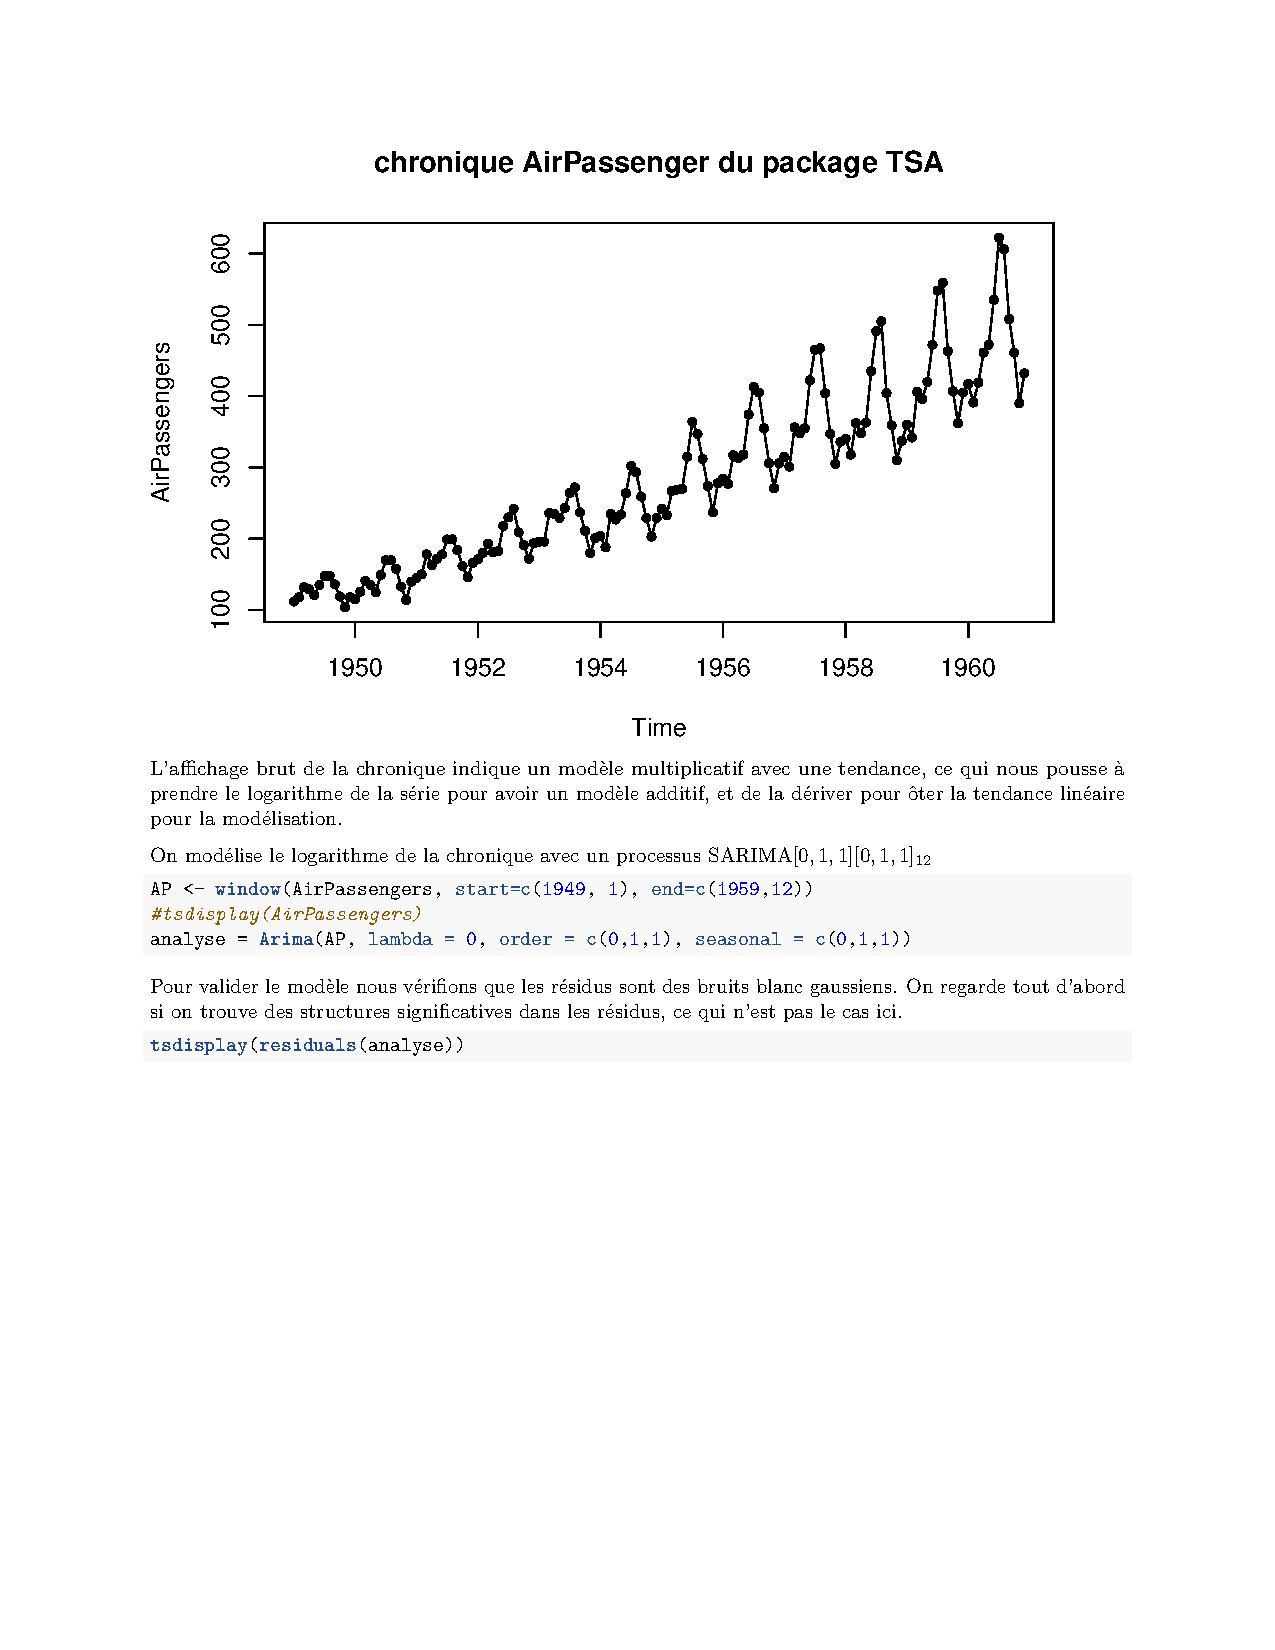
\includepdf[pages=-,pagecommand={\thispagestyle{plain}}]{../R_scripts/SARIMA.pdf}






%%%%%%%%%%%%%%%%%%%%%%%%%%%%%%%%%%%%%%%%%%%%%%%%%%%%%%%%%%%%%%%%%%%%%%%%%%%%%%%%%%%%%%%%%%%%%%%%%%%%%%%%%%%
%%%%%%%%%%%%%%%%%%%%%%%%%%  Approche Bayesienne %%%%%%%%%%%%%%%%%%%%%%%%%%%%%%%%%%%%%%%%%%%%%%%%%%%%%%%%%%%
%%%%%%%%%%%%%%%%%%%%%%%%%%%%%%%%%%%%%%%%%%%%%%%%%%%%%%%%%%%%%%%%%%%%%%%%%%%%%%%%%%%%%%%%%%%%%%%%%%%%%%%%%%%

\section{Approche Bayésienne}

\paragraph{}
Nous allons dans cette partie adopter une approche bayésienne.
Pour des observations $X$ l'approche bayésienne considère pour déterminer les paramètres $\theta$ d'un modèle la distribution de probabilité des 
paramètres postérieure $p(\theta | X)$ en se basant sur la formule de Bayes
\[
	\begin{aligned}
		p(\theta | X) &= \frac{p(X | \theta) p(\theta)}{p(X)} \\
		&= \frac{p(X | \theta) p(\theta)}{\int_{\theta} p(X | \theta) p(\theta) d \theta}	
	\end{aligned}
	\] 
	Avec $p(\theta)$ la probabilité à priori des paramètres. 
	Dans l'approche fréquentiste précédente nous maximisions la vraisemblance $p(X | \theta)$.
	\paragraph{}
	Pour déterminer le $\theta$ optimal $\hat{\theta}$ dans l'approche bayésienne nous utilisons une fonction de coût L$(\cdot\ ,\cdot)$
	et le risque bayésien $R_B(X,{\theta}^\prime)$ 
	\[
		R_B(y,\theta^\prime) = \int_{\Theta} \text{L}(\theta, \theta^\prime) \pi(\theta | X) \mathrm{d} \theta
		\]
		
		\begin{equation}
			\hat{\theta}=\arg \min _{\theta^\prime \in \Theta} R_B(y,\theta^\prime)
		\end{equation}   
		On prend communément L$(\theta,\theta^\prime) = \left\|\theta-\theta^{\prime}\right\|^{2}$ ce qui donne pour $\hat{\theta}$
		$$
		\hat{\theta}=\mathrm{E}[{\theta} | y]
		$$
		\paragraph{}
		Nous utilisons cette distribution à postériori pour établir une distribution pour la prédiction d'observations futures $X^{new}$.

		\begin{equation}
			{p}\left(X^{\text {new }} | {X}\right)=\int_{\theta} {p}\left(X^{\text {new }} | \theta\right) \cdot {p}(\theta | {X}) d \theta
		\end{equation}
		
		\paragraph{}
		Dans la réalité la probabilité postérieure ne pouvant être exprimée simplement, nous allons voir une méthode permettant de simuler
		la probabilité postérieure.
		
%%%%%%%%%%%%%%%%%%%%%%%%%%%%%%%%%%%%%%%%%%%%%%%%%%%%%%%%%%%%%%%%%%%%%%%%%%%%%%%%%%%%%%%%%%%%%%%%%%%%%%%%%%%
\subsection{Méthode de Monté-Carlo et Échantillonnage de Gibbs}
%%%%%%%%%%%%%%%%%%%%%%%%%%%%%%%%%%%%%%%%%%%%%%%%%%%%%%%%%%%%%%%%%%%%%%%%%%%%%%%%%%%%%%%%%%%%%%%%%%%%%%%%%%%

\paragraph{}
La méthode MCMC \textit{Markov Chain Monte Carlo} utilise les propriétés ergodiques des chaînes de Markov 
et la méthode de Monté-Carlo pour estimer une densité de probabilité jointe de variables aléatoires  $\pi(U_1, \ldots, U_K)$
que l'on ne peut obtenir analytiquement.

\paragraph{}
On se place dans le cas où nous pouvons définir les lois conditionnelles entre les variable $U_i$
dont on souhaite connaître la loi jointe avec les lois conditionnelles entre ces variables 
${Loi}(U_j|U_1, \ldots, U_{j-1}, U_j, \dots, U_K)$. \\ En tirant successivement les variables selon leur loi conditionnelle 
on construit une ainsi une chaîne de Markov dont la loi stationnaire est la distribution jointe des variables.    
\paragraph{}
Nous pouvons ainsi après des tirages successif obtenir des tirages $(U_1, \ldots, U_K)$ selon la loi jointe ce qui nous permet 
de faire des estimations selon la méthode de Monté-Carlo.
\paragraph{}
Dans la suite nous rappelons les principes de la méthode de Monté-Carlo et des chaînes de Markov, pour présenter 
l'échantillonneur de Gibbs utilisé pour réaliser les tirages.

\paragraph{Méthode de Monté Carlo \\}
La méthode de Monté-Carlo permet d'obtenir asymptotiquement l'espérance d'une variable aléatoire $X$ 
en effectuant $n$ tirages selon la loi de $X$.
$$
\begin{aligned}
	&\mathbb{E}[f(x)]=\int f(x) p(x) d x \approx \frac{1}{n} \sum_{i=1}^{n} f\left(x^{i}\right) \\
	&\text{où les } (x^i) \text{ sont des tirages indépendants selon la loi de } X 
\end{aligned}
$$
Habituellement utilisée pour estimer des intégrales, nous utilisons la méthode de Monté-Carlo pour estimer des lois de 
variables aléatoires dont nous ne disposons pas d'expression analytique.   

\paragraph{Chaîne de Markov \\}

% Soit un espace d'état $(E,\mathcal{E)$ mesurable avec $\mathcal{E} = \mathcal{P}(E)$. 
% Soit un espace de probabilité $(\Gamma, \mathcal{A}, \mathbb{P})$ })$.
Soit $(X_n)_{n \in \mathbb{}{N}}$ une suite de variable aléatoire définies sur $(\Gamma , \mathcal{A}, \mathbb{P})$ à valeur dans 
$(E, \mathcal{E})$. \\

La suite $(X_n)_{n \in \mathbb{N}}$ est une chaîne de Markov sur $(\Gamma, \mathcal{A}, \mathbb{P})$ si elle vérifie pour 
$\forall n \in \mathbb{N}$, $\forall (x_0, \ldots, x_n) \in E | \mathbb{P}(X_n = x_n, \ldots, X_0 = x_0) > 0$,
\[
	\forall n \in \mathbb{N} \quad \mathbb{P}(X_{n+1}  = x_{n+1} | X_0 = x_1, \ldots, X_n = x_n) = 
	\mathbb{P}(X_{n+1} = x_{n+1}| X_n = x_n)
\]
En particulier $(X_n)_{n \in \mathbb{N}}$ est une chaîne de Markov homogène si elle vérifie 
\[
	\forall i,j \in I \quad \mathbb{P}(X_{n+1}  = x_{j}| X_n = x_i) = P(x_i,x_{j})
\]
Avec $P$ la probabilité de transition.
\paragraph{}
Une mesure positive $v$ sur $(E,\mathcal{E})$ est invariante pour la chaîne $X$ si
\[
	\forall y \in E  \quad v(y) = \sum_{x \in E} P(x,y) v(x)
\]
Si $X$ est une chaîne irréductible récurrente elle admet une unique mesure invariante $v$ avec notamment 
$$ \text{Pour }x \in E, \ \forall y \in E, \quad v(y) = \lim _{n \rightarrow+\infty} P^n
(x,y) $$

De plus avec les théorèmes ergodiques nous avons le résultat suivant pour une mesure invariante $v$ et pour une fonction $f$ $-v$ mesurable 
\begin{equation}
	\lim _{n \rightarrow+\infty} \frac{1}{n} \sum_{i=1}^{n} f\left(X_i\right)=\sum_{x \in E}{f(x) v(x)} 
	\end{equation}
 
\paragraph{Algorithme d'echantillonage de Gibs \\}
\begin{itemize}[label={}]
\item \begin{enumerate}
	\item Prendre des valeur initiales $U^{(0)}_k$, pour $k = 1, \ldots, K$.
	\item Pour $t = 1, 2, \ldots$ :
	\begin{itemize}[label={}]
		\item Pour $k = 1,2, \ldots, K$:
		\begin{itemize}[label={}]
			\item tirer $U_k^{(t+1)}$ depuis la distribution 
			$\operatorname{\pi}(U_{k} | U_{1}^{(t+1)}, \ldots, U_{k-1}^{(t+1)}, U_{k+1}^{(t)}, \ldots, U_{K}^{(t)})$ 
		\end{itemize}
	\end{itemize}
	\item Continuer l'étape 2 jusqu'à convergence de la distribution jointe
	$\pi (U_{1}^{(t)}, U_{2}^{(t)}, \ldots, U_{K}^{(t)})$	
\end{enumerate}
\end{itemize}
\paragraph{}

\paragraph{}
On note pour $x \in E$ avec $x=(x_1,\ldots,x_K)$, $x_{-i} = (x_1, \ldots,x_{i-1},x_{i+1}, \ldots, x_K)$ \\
Soit $x$, $y$ $\in E$. On note $x \underset{j}{\sim} y  \Longleftrightarrow x_{i}=y_{i} \quad \forall i \neq j$ \\
La loi conditionnelle entre les états dans l'échantillonnage de Gibbs est alors (le dénominateur ne dépend plus de $x_i$)
% $$
% \pi(x_{i} | x_{-i})= \frac{\pi(x)}{  \underset{z \in E,x \underset{i}{\sim} z } \int \pi(z)dz}
% $$
$$
\pi(x_{i} | x_{-i})= \frac{\pi(x)}{\pi(x_{-i})}
$$
La probabilité de transition entre deux état $x$ et $y$ est 
$$
P(x,y)=\left\{\begin{array}{ll}
{\pi(y_{i} | x_{-i})} & {\text{si } \exists i\ |\ x \underset{i}{\sim} y }\\
 {0} & {\text { sinon }}
\end{array}\right.
$$
La chaîne de Markov ainsi définie est irréductible comme tous ces états sont communiquants au bout d'un nombre finis d'étapes.
 Elle est de plus apériodique comme $P(x,x)>0$. Cela nous assure l'unicité de la mesure stationnaire de masse finie \cite{wiki}.
\paragraph{}
On vérifie ainsi que $\pi$ est une probabilité d'une chaîne réversible.
$$
\begin{aligned}
	\text{Si } \ x \underset{i}{\sim} y \quad \pi(x) P(x,y) &= \pi(x_i,x_{-i})\ \frac{\pi(y_i, x_{-i})}{\pi(x_{-i})}  \\
	& = \pi(y_i,x_{-i})\ \frac{\pi(x_i, x_{-i})}{\pi(x_{-i})} \\ 
	&= \pi(y) P(y,x) 
\end{aligned}
$$
Ainsi la distribution jointe $\pi$ est la probabilité stationnaire de la chaîne.

\paragraph{}
On peut ainsi estimer la probabilité marginale $\hat{p}$ d'une variable en utilisant l'échantillonnage $(U_1^{(t)},U_2^{(t)},\ldots,U_K^{(t)})$ 
\[
\widehat{\operatorname{p}}_{U_{i}}(y)= \frac{1}
	{(M-m+1)} \sum_{t=m}^{M} \pi (U_i | U_1, \ldots, U_{i-1}, U_{i+1}, \ldots, U_K)
\]
\paragraph{}

On prend en effet les échantillons qu'après $m$ itérations pour que la distribution converge vers la probabilité stationnaire 
de la chaîne de Markov (\textit{burn-in}). $m$ dépend de la vitesse de convergence.\\

De plus les tirages succéssifs de l'échantillonneur de Gibbs sont corrélés. Dans la pratique nous ne prenons également que des tirages  
$\left(U_{1}^{(t)}, U_{2}^{(t)}, \ldots, U_{K}^{(t)}\right)$ espacés d'un \textit{lag} pour obtenir des échantillons indépendants.
On peur regarder le corrélogramme et le corrélograme partiel de l'échantillon pour déterminer le \textit{lag}. \\
Plus les échantillons sont corrélés entre eux, plus nous devons faire de simulations. 
\paragraph{}
On peut s'intéresser à la variance d'un tel estimateur. Dans \cite{coursgibbs} on montre que la variance de l'estimateur dépend
des autocorrélations entre les échantillons de la série généré par l'échantillonneur. 
Ainsi pour un estimateur 
\begin{equation}
	\hat{\mu}=\frac{1}{N} \sum_{n=1}^{N} f\left(X_{n}\right)
\end{equation}
\begin{equation}
	\operatorname{Var}(\hat{\mu}) \approx \frac{\sigma(f)^{2} \tau(f)}{N}
	\end{equation}
Avec $\sigma(f)^{2}$ la variance de $f(X)$ pour la distribution stationnaire et $$\tau=1+2 \sum_{k=1}^{\infty} \rho(k) $$ 
le \og{}temps d'autocorrélation \fg. On a donc intérêt à diminuer les corrélations entre les tirages pour réduire la variance de l'estimateur.
on peut fournir un nombre optimal du nombre de tirages effectués en fonction de $\tau$.
Pour N échantillons on peut mesure l'influence des autocorrections avec la taille effective d'échantillonnage
$ESS = \frac{N}{\tau}$. Cela revient à estimer l'erreur de Monté-carlo de la méthode par $\frac{\sigma(f)^{2}}{ESS}$ 
au lieu de $\frac{\sigma(f)^{2}}{N}$. 

\paragraph{}
Par ailleurs la méthode MCMC présente comme risque de ne pas explorer toutes les valeurs de la loi que l'on souhaite estimer. 
En effet par l'aspect aléatoire certaines valeurs de la loi peuvent ne pas être explorées. Pour contrer cela on peut augmenter le nombre de simulations 
et lancer plusieurs simulations avec des initialisation différentes. 
\paragraph{}
Nous allons utiliser la méthode MCMC dans la suite pour tirer des échantillons des lois postérieures $p(\theta|X)$ pour les paramètres que l'on souhaite estimer.
%%%%%%%%%%%%%%%%%%%%%%%%%%%%%%%%%%%%%%%%%%%%%%%%%%%%%%%%%%%%%%%%%%%%%%%%%%%%%%%%%%%%%%%%%%%%%%%%%%%%%%%%%%%
\subsection{Le modèle d'espace d'état}
%%%%%%%%%%%%%%%%%%%%%%%%%%%%%%%%%%%%%%%%%%%%%%%%%%%%%%%%%%%%%%%%%%%%%%%%%%%%%%%%%%%%%%%%%%%%%%%%%%%%%%%%%%%


\paragraph{}
Une généralisation des modèles employés pour la modélisation des séries temporelles s'écrit :

\begin{equation}
	\label{obeservationeq}
	y_{t}=Z_{t}^{T} \alpha_{t}+\epsilon_{t} \quad \epsilon_{t} \sim \mathcal{N}\left(0, H_{t}\right)
\end{equation}
\begin{equation}
	\label{transitioneq}
	\alpha_{t+1}=T_{t} \alpha_{t}+R_{t} \eta_{t} \quad \eta_{t} \sim \mathcal{N}\left(0, Q_{t}\right)
\end{equation}
\vspace{0.1cm}
\[
	\begin{aligned}
		& \text{avec} \ Z_t, \ H_t , \ T_t, \ R_t, \ Q_t \ \text{des matrices à déterminer}. \\
		& \epsilon_t\text{ indépendants, }\eta_t\text{ indépendants} \\
		& (y_t,\epsilon_t)\text{ indépendants,  }(\alpha_t,\eta_t)\text{ indépendants}
	\end{aligned}
\]
	
\ref{obeservationeq} est l'équation dite d'\textit{observation} car elle corresponds aux états de la série temporelle observables. 
\ref{transitioneq} est l'equation dite de \textit{transition} car elle correspond à des états non visibles de façon similaire à un modèle de Markov caché. 
La combinaison de ces deux équations forme un modèle espace d'état (\textit{state space form model}) sous sa forme gaussienne linéaire. On peut notamment dériver un modèle $ARIMA$ de ce modèle général.

\paragraph{}

Le modèle bayésien classique utilisé dans \cite{pedictbayesian} s'exprime de la manière suivante :

\begin{equation}
	\label{modelebayes}
	\begin{aligned} 
		y_{t} &=\mu_{t}+\tau_{t}+\beta^{T} \mathbf{x}_{t}+\epsilon_{t} \quad & \epsilon_{t} 
		\sim \mathcal{N}(0, \sigma_{\epsilon}^2) \\ 
		\mu_{t} &=\mu_{t-1}+\delta_{t-1}+u_{t} \quad & u_{t} \sim \mathcal{N}(0, \sigma_{u}^2) \\
		\delta_{t} &=\delta_{t-1}+v_{t} \quad & v_{t} \sim \mathcal{N}(0, \sigma_{v}^2) \\
		\tau_{t} &=-\sum_{s=1}^{S-1} \tau_{t-s}+w_{t} \quad & w_{t} \sim \mathcal{N}(0, \sigma_{w}^2)
	\end{aligned}
\end{equation}

On peut exprimer \ref{modelebayes} avec \ref{obeservationeq} avec un terme de régression comme dans \cite{kapman1993} 
(S .J. Koopman 1993) \\
On omet la composante saisonnière $\tau_{t}$, traitée à part, qui ne sera pas pris en compte dans le modèle final car les données sont 
\og désaisonnalisées \fg{}.

\begin{equation}
\begin{aligned} y_{t} &= Z_{t} \alpha_{t}+ \varepsilon_{t}\\ 
\alpha_{t+1} &= T_{t} \alpha_{t}+ \varepsilon_{t}
\end{aligned}
\end{equation}
Avec 
\[
\begin{aligned}
	Z_{t}^{T} &= (\begin{array}{lll}{1} & {0} & {\beta^{T} \mathbf{x}_{t}}\end{array}), \
	H_t = \sigma_{\epsilon}^{2} \in \mathbb{R}^{+*} \\
\alpha_{t} &= \left(\begin{array}{c}{\mu_{t}} \\ {\delta_{t}} \\ {1}\end{array}\right) , \
T_t = \left(\begin{array}{lll}{1} & {1} & {0} \\ {0} & {1} & {0} \\ {0} & {0} & {1}\end{array}\right) \\
Q_t &= \left(
	\begin{array}{lll}{
		\sigma_{u}^{2}} & {0} & {0} \\
		 {0} & {\sigma_{v}^{2}} & {0} \\
		  {0} & {0} & {\sigma_{w}^{2}}
	\end{array}
	\right), 
R_{t} = \left(\begin{array}{lll}{1} & {0} & {0} \\ {0} & {1} & {0} \\ {0} & {0} & {0}\end{array}\right),
\eta_{t} = \left(\begin{array}{c}{u_{t}} \\ {v_{t}} \\ {w_t}\end{array}\right)
\end{aligned}
\]
Si on inclut le terme saisonnal $\tau$ on a 
$\alpha_{t}^{T} = (\begin{array}{llllll}{\mu_{t}} & {\delta_{t}} & {\tau_{t}} & {\tau_{t-1}} & ...&  {\tau_{t-S+1}}\end{array})$

\paragraph{}
Nous allons décrire les méthodes pour obtenir les paramètre du modèle ainsi définis. C'est à dire les méthodes dans une approche bayésienne
nous permettant avec une distribution à priori des paramètres, obtenir la distribution à postériori.
Tous d'abord nous allons présenter le filtre de Kapman afin d'obtenir les états cachés $\alpha_T$ puis l'implémentaion de l'échantilloneur de gibbs afin
d'obtenir la distribution postérieure pour $\beta$.

%%%%%%%%%%%%%%%%%%%%%%%%%%%%%%%%%%%%%%%%%%%%%%%%%%%%%%%%%%%%%%%%%%%%%%%%%%%%%%%%%%%%%%%%%%%%%%%%%%%%%%%%%%%
\subsection{Filtre de Kapman}
%%%%%%%%%%%%%%%%%%%%%%%%%%%%%%%%%%%%%%%%%%%%%%%%%%%%%%%%%%%%%%%%%%%%%%%%%%%%%%%%%%%%%%%%%%%%%%%%%%%%%%%%%%%

\paragraph{}
On veut déterminer dans cette partie les états \og{} caché \fg $ \alpha_t$ dit aussi latents. \\
Les $\alpha_t$ peuvent être vus comme les états caché d'une chaîne de Markov caché dont les états observables sont les $y_i$
On détermine les $\alpha_t$ par l'utilisation du filtrage et du lissage de Kalman \cite{kalman}.

\paragraph{}
On veut déterminer $\alpha_t$, $H_t$ et $Q_t$ ($H_t,Q_t$ constant en pratique) à partir des
observations  $y_{1: t} = y_1, y_2, ..., y_t$.
On suppose connu $\beta$.
\paragraph{}
Le principe de filtrage est obtenu par la linéarité des variables gaussiennes dans \ref{obeservationeq} et \ref{transitioneq} 
$p(\alpha_{t} | y_{1: t}) \sim \mathcal{N}(\hat{\alpha}_{t}, P_t)$.
Avec ainsi $\hat{\alpha}_{t} = \mathrm{E}(\alpha_{t} | y_{1:T})$ et 
$P_{t} = E\left[\left(\alpha_{t}-\hat{\alpha}_{t}\right)\left(\alpha_{t}-\hat{\alpha}_{t}\right)^{T}\right]$
\paragraph{}
Pour effectuer un tirage selon la loi $p(\alpha_{t} | y_{1:t})$ on effectue un tirage $\alpha_t^+$ selon la probabilité 
à priori $p(\alpha)$ 
et on prend $\hat{\alpha}_t^+ = E(\alpha_{t}^+ | y_{1:t}^+)$. \\
Ainsi $\tilde{\alpha}_t = \hat{\alpha}_t - \hat{\alpha}_t^+ + \alpha_t^+$ est un tirage selon $p(\alpha_{t} | y_{1: t})$
\paragraph{}
Le filtre de base pour estimer le bruit gaussien des
$\left(\begin{array}{c}{
    \varepsilon_t} \\ 
{\eta}_t\end{array}
\right)$
en itérant sur $t=1, \ldots, T$
est donné par \cite{kalman}  : 
\begin{equation}
	\begin{aligned}
        &a_{t+1} =E(\alpha_{t+1} | y_{1:t}) = T_{t} a_{t}+K_{t} v_{t}\\
        &v_{t} = y_{t}-E(y_{t} |y_{1: t-1}) = y_{t}-Z_{t} a_{t}  \\
        &P_{t+1} = T_{t} P_{t} L_{t}^{T}+R_{t} Q_{t} R_{t}^{T} \\
        &F_{t} = \operatorname{Var}\left(v_{t}\right)=Z_{t} P_{t} Z_{t}^{\prime}+H_{t} \\
	&K_{t} =T_{t} P_{t} Z_{t}^{T} F_{t}^{-1} \\
	&L_{t}=T_{t}-K_{t} Z_{t} \\
	&\left(
        \begin{array}{c}{
            \hat{\varepsilon}_t} \\ 
            {\hat{\eta}_t}
        \end{array}
        \right)
        = \left[
            \begin{array}{cc}{
                H_{t} F_{t}^{-1}} & {-H_{t} K_{t}^{T}} \\
                {0} & {Q_{t} R_{t}^{T}}
            \end{array}\right]
            \left(
                \begin{array}{c}{
                    v_{t}} \\
                    {r_{t}}
                \end{array}
                \right)
            \end{aligned}
        \end{equation}
        avec $r_t$ évalué rétrospectivement sur $t=T, \ldots, 1$:
        \begin{equation}
            \label{backward}
            \begin{aligned}
                &r_{t-1} =Z_{t} F_{t}^{-1} v_{t}+L_{t}^{T} r_{t}\text{  pour  } t=T, \ldots, 1 \\
                &r_T = 0
            \end{aligned}
        \end{equation}
        Ainsi on peut itérer les $\hat{\alpha}_{t+1}$ sur $t=1, \ldots, T$
\begin{equation}
    \label{forward}
    \begin{aligned}
		\hat{\alpha}_{t+1}&=\mathrm{E}\left(\alpha_{t} | y_{1: T}\right) \\
		 &= T_{t} \hat{\alpha}_{t}+R_{t}\hat{\eta}_t \\
        &= T_{t} \hat{\alpha}_{t}+R_{t} Q_{t} R_{t}^{T} r_{t}\\
        \text{avec }\hat{\alpha}_{1} &= a_{1}+P_{1} r_{0}
    \end{aligned}
\end{equation}

\paragraph{}
L'algorithme pour obtenir le tirage $\tilde{\alpha}$ est le suivant:
\begin{itemize}[label={$\bullet$}]
\item On tire le vecteur des perturbations  $\left(\begin{array}{c}{
    \varepsilon_t^+} \\ 
    {\eta^+}_t\end{array}
    \right)$   
selon la distribution à priori avec $H_t$ et $Q_t$. On tire $\alpha_{1}^{+} \sim \mathrm{N}\left(a_{1}, P_{1}\right)$ et ainsi 
itérativement sur \ref{obeservationeq} en prenant la moyenne on obtient $\alpha^+$ et $y^+$.
\item Avec \ref{forward} et \ref{backward} on obtient $\hat{\alpha}$ et en prenant la moyenne $\hat{\alpha}^+$.
\item On obtient ainsi $\tilde{\alpha}=\hat{\alpha}-\hat{\alpha}^{+}+\alpha^{+}$
\end{itemize}

\paragraph{}
On peut séparer la procédure précédente en deux éléments : le filtre de Kalman et le lissage de Kalman.

\paragraph{Filtre de Kalman}
\begin{itemize}
\item On itère en avant de 1 à $T$.
\item On combine $p\left(\alpha_{t} | y_{1: t}\right)$ et $y_t$ pour avoir $p\left(\alpha_{t+1} | y_{1: t}\right)$
\end{itemize}

\paragraph{Lissage de Kalman}
\begin{itemize}
    \item On itère en arrière de T à 1
    \item On combine $r_t$ et $p\left(\alpha_{t+1} | y_{1: t}\right)$ pour obtenir $p\left(\alpha_{t+1} | y_{1: T}\right)$
\end{itemize}


%%%%%%%%%%%%%%%%%%%%%%%%%%%%%%%%%%%%%%%%%%%%%%%%%%%%%%%%%%%%%%%%%%%%%%%%%%%%%%%%%%%%%%%%%%%%%%%%%%%%%%%%%%%
\subsection{Utilisation d'une loi à priori \textit{spike and slab}}
%%%%%%%%%%%%%%%%%%%%%%%%%%%%%%%%%%%%%%%%%%%%%%%%%%%%%%%%%%%%%%%%%%%%%%%%%%%%%%%%%%%%%%%%%%%%%%%%%%%%%%%%%%%
\paragraph{}
Nous mettons en place une méthode de séléction de variable similaire à la regression ridge pour \og{} mettre à zéro \fg{}  certains paramètres de la régression. Ceci permet notamment 
de prendre en compte les corrélations entre les variables explicatives du modèle et de réduire la taille du modèle.

\paragraph{}
Cette selection se fait sur la probabilté à priori de $\beta$ en utilisant une loi 
variable aléatoire $\gamma$ qui suit une loi de Bernoulli. \\

\paragraph{Les distributions à priori \\}
On definie ainsi la \textit{spike and slab prior}:

\begin{equation}
	p\left(\beta, \gamma, \sigma_{\varepsilon}^{2}\right)=p\left(\beta_{\gamma} | \gamma, \sigma_{\varepsilon}^{2}\right) p\left(\sigma_{\varepsilon}^{2} | \gamma\right) p(\gamma)
\end{equation}
$\gamma$ ayant pour distribution à priori avec $K$ le nombre de variable explicatives.
\begin{equation}
	p(\gamma)=\prod_{k=1}^{K} \pi_k^{\gamma k}(1-\pi_k)^{1-\gamma k}
\end{equation}
Les $\pi_k$ peuvent être pris constants $ \forall k$, à 0 ou 1 si on veut exclure ou inclure certaines variables. On peut ausi
si on souhaite avoir un modèle de taille $p$ poser $\pi = \frac{p}{K}$

\paragraph{}
On a également les probabilités à priori
\[
	\beta_{\gamma}\left|\sigma_{\epsilon}^{2}, \gamma \sim \mathcal{N}\left(b_{\gamma},
	\sigma_{\epsilon}^{2}\left(\Omega_{\gamma}^{-1}\right)^{-1}\right) \quad \sigma_{\epsilon}^{2}\right| \gamma \sim IG\left(\frac{\nu}{2}, \frac{s s}{2}\right)
	\]
	Avec $IG(.,.)$ la distribution Gamma inverse, s$\Omega^{-1}\propto X^{T} X$ similairement à la méthode des moindre carrés. $\Omega_{\gamma}$ est la matrice $\Omega$
	pour les rangs et colonnes $k$ tel que $\gamma_k  = 1$  
	
	\begin{equation}
		\frac{s s}{d f}=\left(1-R^{2}\right) s_{y}^{2}
	\end{equation}
	Avec $R^2$ le coéfficent de détermination attendu de la régression, et $s_{y}$ l'ecart quadratique moyen de la regression.
	
\paragraph{Les distributions à postériori \\}
On prend $y_t$ de \ref{obeservationeq} en omettant la partie serie temporelle avec $y_{t}^{*}$ pour ne garder que la partie de regression\\ 
$y_{t}^{*}=y_{t}-Z_{t}^{* T} \alpha_{t} = y_{t}-{Z_{t}^{T}}_{ | \beta \mathbf{x}_t = 0} \ \alpha_{t} = y_t - \mu_t$ \\
On prend $$\mathrm{y}^{*}=y_{\mathrm{1:n}}^{*}$$

\paragraph{}
On a alors les résultats suivants pour les lois à postériori
\begin{equation}
	\beta_{\gamma}\left|\sigma_{\epsilon}, \gamma, \mathbf{y}^{*} \sim \mathcal{N}\left(\tilde{\beta}_{\gamma}, 
	\sigma_{\epsilon}^{2}\left(V_{\gamma}^{-1}\right)^{-1}\right) \quad 
	{\epsilon}^{2}\right| \gamma, \mathbf{y}^{*} \sim IG\left(\frac{\nu+n}{2}, \frac{S S_{\gamma}}{2}\right)
\end{equation}
Avec 
\begin{equation}
\begin{aligned}
V_{\gamma}^{-1} &=\left(\mathbf{X}^{T} \mathbf{X}\right)_{\gamma}+\Omega_{\gamma}^{-1} \\
 \tilde{\beta}_{\gamma} &=\left(V_{\gamma}^{-1}\right)^{-1}\left(\mathbf{X}_{\gamma}^{T} \mathbf{y}^{*}+\Omega_{\gamma}^{-1} b_{\gamma}\right) \\ 
SS_{\gamma}& =ss+\mathbf{y}^{* T} \mathbf{y}^{*}+b_{\gamma}^{T} \Omega_{\gamma}^{-1} b_{\gamma}-\tilde{\beta}_{\gamma}^{T} V_{\gamma}^{-1} \tilde{\beta}_{\gamma}
\end{aligned}
\end{equation}

En utilisant les distributions postérieures et en marginalisant on trouve la distribution postérieure:
\begin{equation}
	\gamma | \mathbf{y}^{*} \sim C\left(\mathbf{y}^{*}\right) \frac{\left|\Omega_{\gamma}^{-1}\right|^{\frac{1}{2}}}{\left|V_{\gamma}^{-1}\right|^{\frac{1}{2}}} \frac{p(\gamma)}{S S_{\gamma}^{\frac{N}{\gamma}-1}}
	\end{equation}
Avec $ C\left(\mathbf{y}^{*}\right)$ une constante de normalisation.

%%%%%%%%%%%%%%%%%%%%%%%%%%%%%%%%%%%%%%%%%%%%%%%%%%%%%%%%%%%%%%%%%%%%%%%%%%%%%%%%%%%%%%%%%%%%%%%%%%%%%%%%%%%
\subsection{Entrainement des paramètres}
%%%%%%%%%%%%%%%%%%%%%%%%%%%%%%%%%%%%%%%%%%%%%%%%%%%%%%%%%%%%%%%%%%%%%%%%%%%%%%%%%%%%%%%%%%%%%%%%%%%%%%%%%%%
\paragraph{}
Pour obtenir la distribution postérieure des paramètres on utilise la méthode MCMC présenté précédemment.
A chaque itération les paramètres tirés des lois à priori permettent de tirer des paramètres selon la loi postérieure.
\paragraph{}
Sur $1, \ldots, M$
On commence par tirer $\gamma, \beta, \sigma_{\varepsilon}^{2}, \sigma_{v}^{2}, \sigma_{u}^{2}$ de leur distribution à priori.
\begin{enumerate}
\item Avec le filtre de Kalman on simule les état latents $\alpha$ depuis $p\left(\alpha | y, \gamma, \beta, \sigma_{\varepsilon}^{2}, \sigma_{v}^{2}, \sigma_{u}^{2}\right)$
\item On simule $\sigma_u^2$ et $\sigma_v^2$ avec la distribution postérieure $p\left(\frac{1}{\sigma_{u}^{2}}, \frac{1}{\sigma_{v}^{2}} | y, \alpha, \beta, \sigma_{\varepsilon}^{2}\right)$
\item On simule $\beta$ et $\sigma_\epsilon^2$ avec la distribution postérieure $p\left(\beta, \sigma_{\varepsilon}^{2} | y, \alpha, \sigma_{u}^{2}, \sigma_{v}^{2}\right)$
\item Retour à la première étape.
\end{enumerate}
\paragraph{}
$\sigma_u^2$,$\sigma_u^2$,$\sigma_w^2$ sont tiré selon la loi $. | \gamma \sim I G\left(\frac{\nu}{2}, \frac{s s}{2}\right)
$
\paragraph{}
Le modèle final est la moyenne des modèles $\left(\gamma, \beta, \sigma_{\varepsilon}^{2}, \sigma_{v}^{2}, \sigma_{u}^{2}\right)_t$ 
ainsi tirés.

\newpage
%%%%%%%%%%%%%%%%%%%%%%%%%%%%%%%%%%%%%%%%%%%%%%%%%%%%%%%%%%%%%%%%%%%%%%%%%%%%%%%%%%%%%%%%%%%%%%%%%%%%%%%%%%%

%%%%%%%%%%%%%%%%%%%%%%%%%%%%%%%%%%%%%%%%%%%%%%%%%%%%%%%%%%%%%%%%%%%%%%%%%%%%%%%%%%%%%%%%%%%%%%%%%%%%%%%%%%%

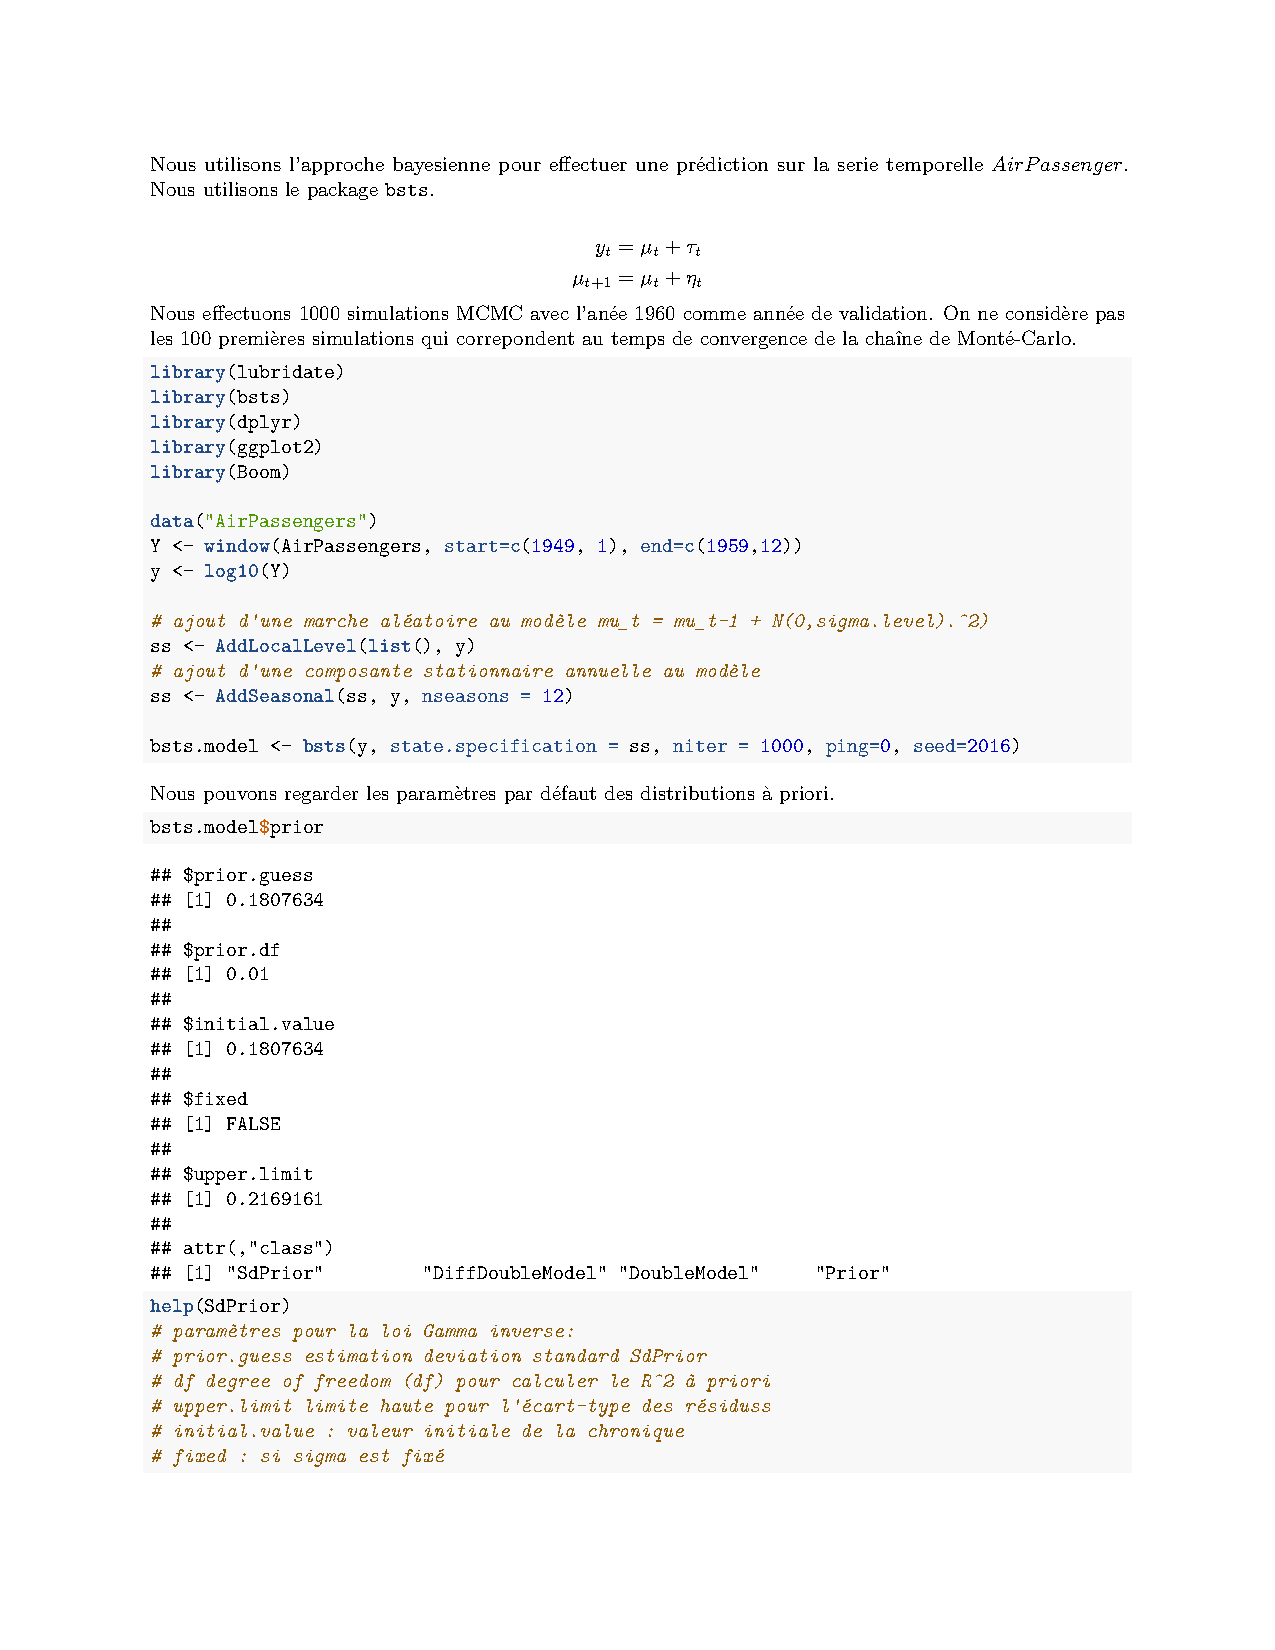
\includepdf[pages=1,pagecommand={
	\section{Utilisation du modèle sur la chronique \textit{AirPassenger}}
	\thispagestyle{plain}}, scale=0.95, offset=0 -1cm]{../R_scripts/Bayesian_Aipassenger.pdf}
\includepdf[pages={2-},pagecommand={
	\thispagestyle{plain}}]{../R_scripts/Bayesian_Aipassenger.pdf}
	
%%%%%%%%%%%%%%%%%%%%%%%%%%%%%%%%%%%%%%%%%%%%%%%%%%%%%%%%%%%%%%%%%%%%%%%%%%%%%%%%%%%%%%%%%%%%%%%%%%%%%%%%%%%

%%%%%%%%%%%%%%%%%%%%%%%%%%%%%%%%%%%%%%%%%%%%%%%%%%%%%%%%%%%%%%%%%%%%%%%%%%%%%%%%%%%%%%%%%%%%%%%%%%%%%%%%%%%


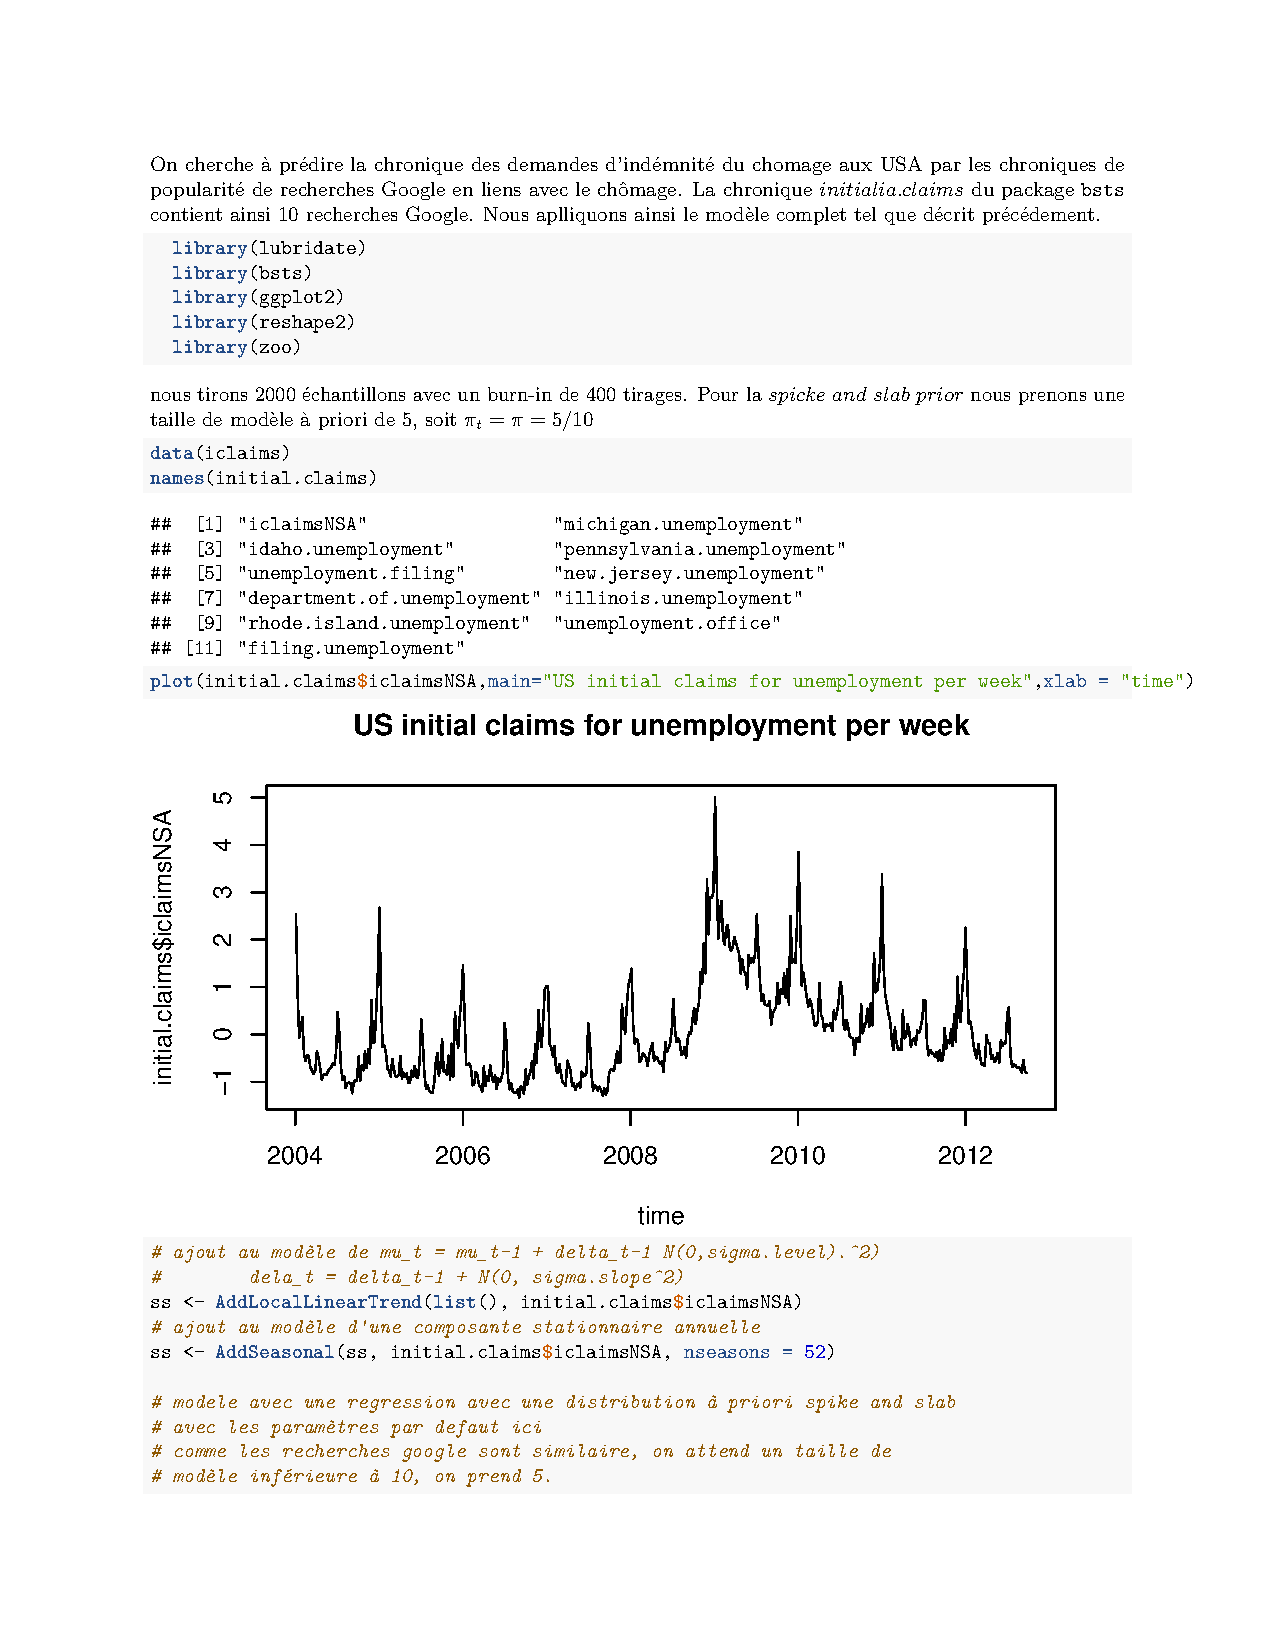
\includepdf[pages=1,pagecommand={
	\section{Prédiction des données du chômage avec la \textit{spike and slab prior}} 
	 \thispagestyle{plain}}, scale=0.95, offset=0 -1cm]{../R_scripts/Full_bayesian_model.pdf}
\includepdf[pages={2-}	,pagecommand={
\thispagestyle{plain}}]{../R_scripts/Full_bayesian_model.pdf}

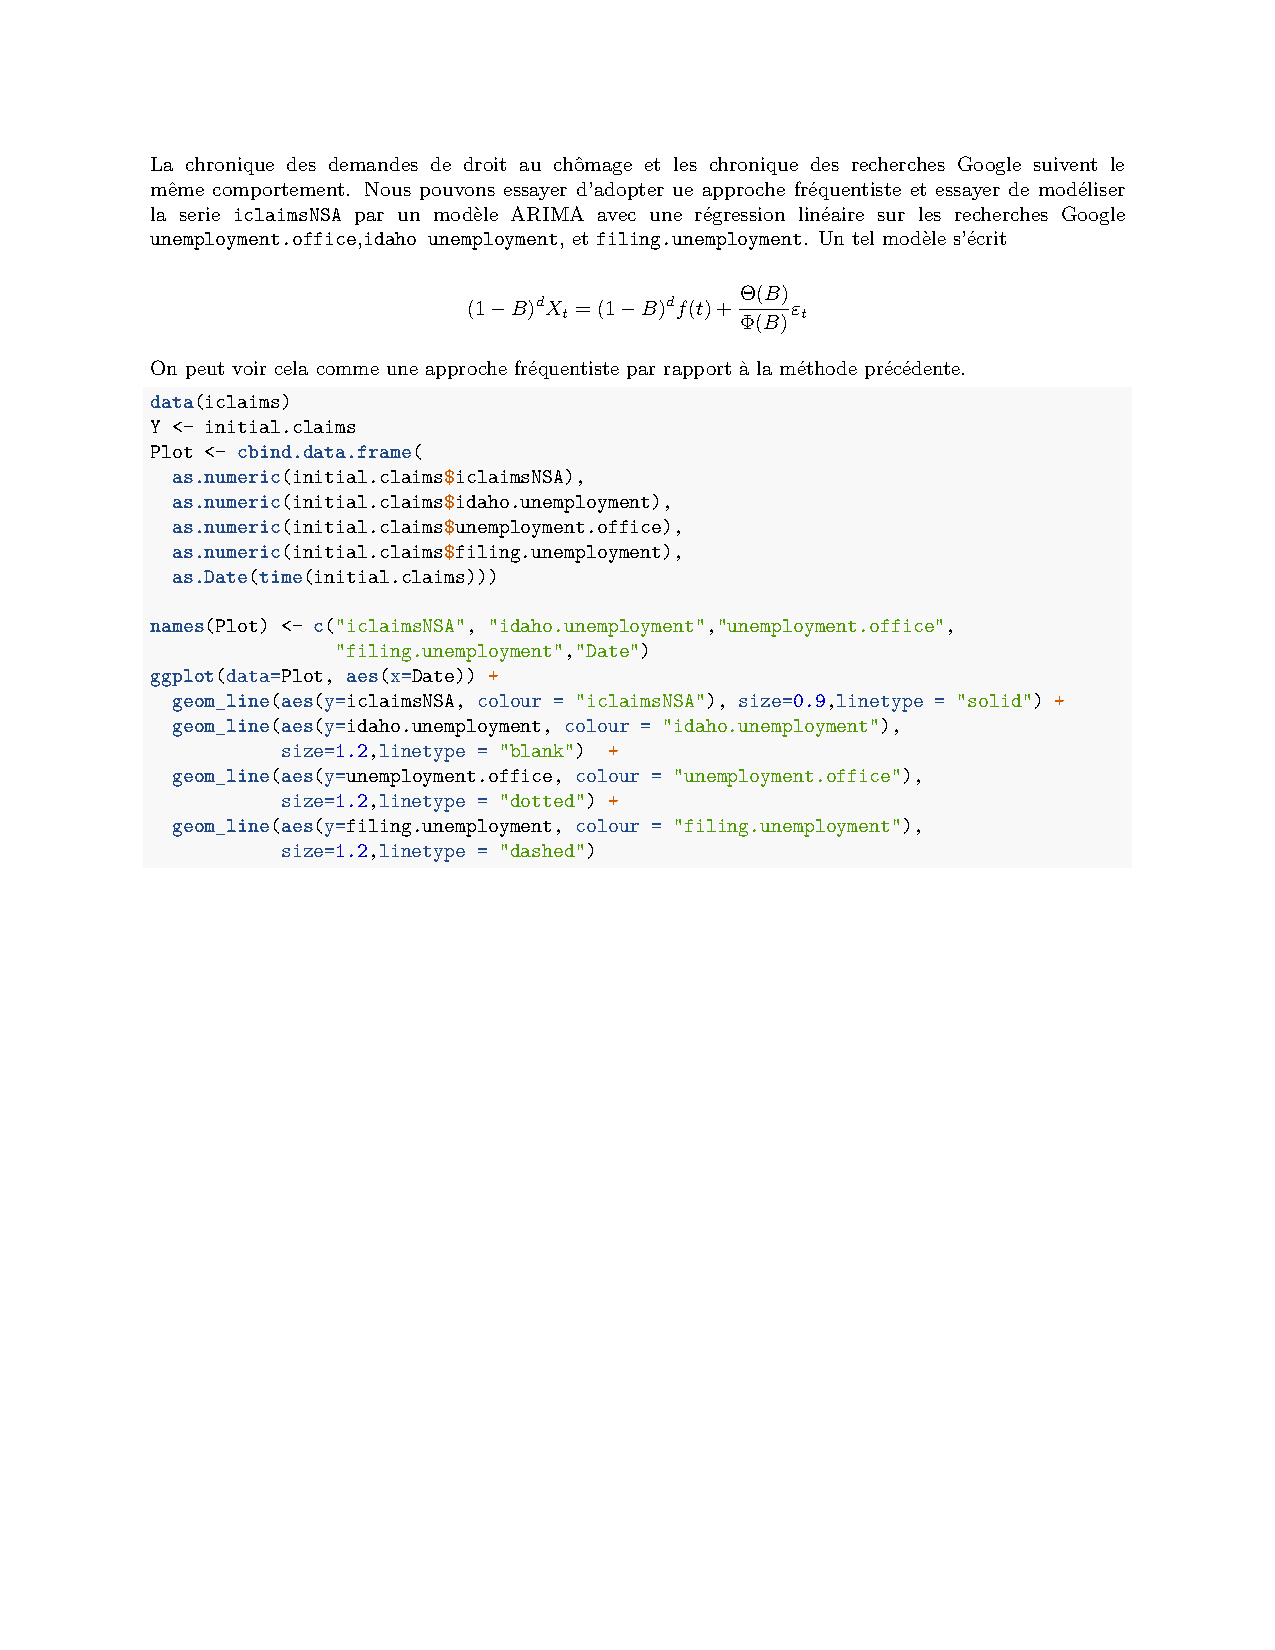
\includepdf[pages={1-},pagecommand={\thispagestyle{plain}}]{../R_scripts/try_arima.pdf}

%%%%%%%%%%%%%%%%%%%%%%%%%%%%%%%%%%%%%%%%%%%%%%%%%%%%%%%%%%%%%%%%%%%%%%%%%%%%%%%%%%%%%%%%%%%%%%%%%%%%%%%%%%%
\section{Comparaison de l'approche bayésienne et de l'approche fréquentiste}
%%%%%%%%%%%%%%%%%%%%%%%%%%%%%%%%%%%%%%%%%%%%%%%%%%%%%%%%%%%%%%%%%%%%%%%%%%%%%%%%%%%%%%%%%%%%%%%%%%%%%%%%%%%
\paragraph{}
Nous pouvons comparer les deux approches que nous avons mit en place : une approche fréquentiste tout d'abord pour estimer les paramètres du modèle
en maximisant la vraissemblance des données. Ensuite l'approche bayésienne où nous posont une estimation à priori qui est actualisée
par les données.
\paragraph{}
Dans le premier cas nous obtenons une estimation directe du paramètre optimal à aplliquer, avec une variance determinée par 
l'information de fisher. Dans le second cas nous obtenons une distribution de probabilité sur laquelle nous effectuons un choix.
\paragraph{}
Le principale reproche fait à l'approche bayésienne est la subjectivité introduite dans le modèle, mais d'une part des modèles de lois 
à priori non-informatives ont été développés et cette subjectivité peut permettre d'éviter des phénomènes
 d'overfitting ou de biais dans l'échantillon des données.
\paragraph{}
D'autre part les intervalles de confiance à postériori semblent plus naturels à utiliser, et permettent de se renseigner sur l'influence des données
sur les hypothèse à priori. Nous avons pu voir comme autre avantage majeure de la méthode est qu'elle n'est pas impacté par des ruptures
de tendances où dans une approche fréquentiste il aurait fallu utiliser des modèles non linéaires plus complexes. De plus les  intervalles 
de confiances pour une prédiction à long terme sont beacoup plus ressérés . 
\paragraph{}
Cependant dans la converge de la méthode MCMC , nous pouvont être induit en erreur sur la convergence du modèle, il est possible 
que certaines valeurs de la distribution à postériori ne soient pas explorées pour cause de probabilités trop faible dans la chaîne de Markov. Il peut 
également être perturbant de considérer que plusieurs simulationss ne renverrons pas les mêmes estimations pour 
les paramètres du modèle de part l'aspect aléatoire de la méthode. De plus l'approche fréquentiste se montre utilise 
pour rejetter des hypothèses sur les données avec des statistiques de test.



\newpage

\textbf{\Huge Conclusion}

\paragraph{}
Nous avons ainsi pu étudier une nouvelle approche statistique pour paramétrer nos modèles. Les méthode de Monté-Carlo par chaîne 
de Markov possèdent de nombreuse autres implémentations que l'algorithme d'échantillonnage de Gibbs que nous avons présenté,
pour une réduction des corrélatins entres les tirages succéssifs et une meilleure exploration de toute les valeurs prises par la chaîne.
Ces méthodes sont le piller de nombreuse applications d'analyse de données comme l'algorithme d'espérence-maximisation 
où l'allocation de Dirichlet latente. Ces méthodes de classification peuvent notamment être implémentées de manière non pararamétriques.























% Comparaison dans l'article  avec la \textit{cumulative absolute forecasting error}
% \begin{equation}
% 	\mathrm{CAFE}=\sum_{i=1}^{n}\left|e_{i}\right|
% \end{equation}

% Utilisation de la méthode de sampling stochastic search variable  selection SSVS dervé de % $MC^{3}$ (─\cite{BAM})

% \section{Compraraison avec méthode de transfert}
% \subsection{Note sorry ARIMA}

% Modèle bayésien classique:
% \begin{equation}
% 	\begin{aligned} Y_{t}=& \mu_{t}+x_{t} \beta+S_{t}+e_{t}, e_{t} \sim N\left(0, \sigma_{e}^{2}\right) \\
%  & \mu_{t+1}=\mu_{t}+\nu_{t}, \nu_{t} \sim N\left(0, \sigma_{\nu}^{2}\right) 
% \end{aligned}
% \end{equation}


% \subsection{Notes article : Predicting the Present with Bayesian Structural Time Series}

% Problèmme : prédire valeur actuelle

% On point positif de l'approche bayesien est que l'on peut voir avec la post probability la contribution de chaque variable explicative ce qui beaoucoup plus transparent
% et clait à percevoir.



% \subsection{Bayesien vs fréquentistes}

% Argument on prefère controler l'incertitude du modèle avec la prior que sur des variables d'ajustement "bizarre" dans ARIMA
% Modèle bayésien non paramétrique car le modèle va s'ajuster aux données avec la prior, pas besoin de calculer la vraisemblance on cherche juste à obtenir la meilleure post probability

% From the point of view of Bayesian inference, MLE is a special case of maximum a posteriori estimation (MAP) that assumes a uniform prior distribution of the parameters.

% And one more difference is that maximum likelihood is overfitting-prone, but if you adopt the Bayesian approach the over-fitting problem can be avoided. 

% L'approche bayésienne permet de moyenner sur des valeurs non observés
% la post est l'actualisation de la prior avec la likelihhodd

% argument our approche bayesiennes :
% - on peut faire des intervalles de confidences des paramètre alors que pour MLE on utilise le ration des likelihood/ wald test
% cette incertitude dans l'estimateur est comprise dans la prédiction
% MCMC permet une meilleur convergence

% MCMC utilise sampling de gibbs pour que la mesure invariante de la suite de Mc suive la distribution jointe 

% Utilisation du package btsts pour le modèle bayésien chinese restaurant process


% utilisation d'un nombre infinin s de gaussienne pour un modèle non paramètrique

% Bayesien contre fréquentiste:
% mail à la liste de diffusion ISBA (internatinnal society for bayesian Analysis)
% \url{http://tonyohagan.co.uk/academic/pdf/HiggsBoson.pdf}
% Les test de Nayman person avec rique alpha et beta e sont pas adaptée à la recherche scientifique pure
% L'inférence baysienne consiste en une croyance exprimé par une probabilité actulisé par l'observation
% (pas dans le cas de l'inforformative prior ou entrpopie maximale)
% L'acceptation de l'hypothèse nulle signifie uniquement que les données n'ont pas réussis à la discréditer
% principle critique du modèle bayesien : subjectivité de la priorf

% Pour comporer les hypothèse facteur de bayse un peu comme facteurde vraissemblance 

% Bayesien et frequentiste divergent quand l'échantillon augmentecar biais


% \subsection{Selection de modèles }

% tilisation pour la sélection de modèle du bayesian model averaging (BAM) \cite{BAM}

% On ne garde que les modèle qui ont une probilité postérieure supérieure à un limite basse.

% \begin{equation}
% \text { (1) } \quad \operatorname{pr}(\Delta | D)=\sum_{k=1}^{K} \operatorname{pr}\left(\Delta | M_{k}, D\right) \operatorname{pr}\left(M_{k} | D\right)
% \end{equation}
% \begin{equation}
% \text { (2) } \quad \operatorname{pr}\left(M_{k} | D\right)=\frac{\operatorname{pr}\left(D | M_{k}\right) \operatorname{pr}\left(M_{k}\right)}{\sum_{l=1}^{K} \operatorname{pr}\left(D | M_{l}\right) \operatorname{pr}\left(M_{l}\right)}
% \end{equation}
% \begin{equation}
% \text { (3) } \quad \operatorname{pr}\left(D | M_{k}\right)=\int \operatorname{pr}\left(D | \theta_{k}, M_{k}\right) \operatorname{pr}\left(\theta_{k} | M_{k}\right) d \theta_{k}
% \end{equation}







\newpage

% You can choose a citation style, 'plain' is the default
% See:
% https://www.overleaf.com/learn/latex/Bibtex_bibliography_styles

\nocite{*}

\bibliography{references.bib}
\bibliographystyle{plain}


\end{document}

% Have fun!
% -fons

% http://www2.washjeff.edu/users/rhigginbottom/latex/resources/symbols.pdfw